\documentclass[../entwurf.tex]{subfiles}
\begin{document}

\section{View}
In dem View Namespace sind die .xaml Dateien, die die UI-Elemente enthalten und die .cs Dateien mit dem Code-Behind des Layouts. Der Wert der UI-Elemente ist mittels Databindig mit dem ViewModel der entsprechenden ViewPage verbunden. Durch Drücken auf die UI-Elemente wird ein Command im ViewModel der zugehörigen ViewPage ausgeführt. 
\subsection{MainPage}
Die MainPage ist die Seite, die direkt beim Start der App angezeigt wird. Bei nicht verbunden Earables wird dem Benutzer ein graues Bluetooth Logo angezeigt. Durch Drücken auf dieses wird zur ConnectionPage gewechselt. Dort kann sich der User mit den Earables verbinden. Bei verbundenen Earables wird dem Benutzer ein blaues Bluetooth Logo und darunter die Schritte angezeigt. Durch Drücken auf das blaue Bluetooth Logo wird die Verbindung zu den Earables getrennt. 

\begin{center}
	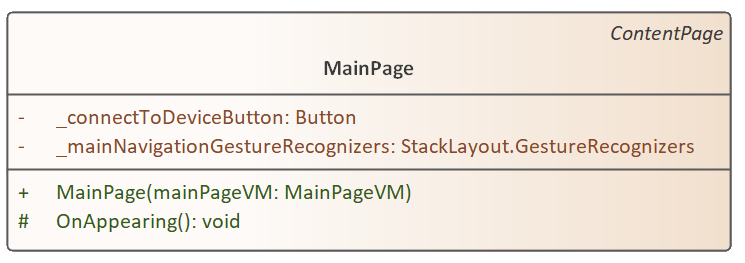
\includegraphics[page=1,width=350pt,keepaspectratio]{../uml_klassen/View/MainPage.png}
\end{center}

\paragraph{Attribute}

\begin{itemize}
	\i{private MainPageVM \_mainPageVM} ViewModel der MainPage
	\i{private StackLayout.GestureRecognizers \_mainNavigationGestureRecognizers} Ist für die Navigation von der MainPage aus zuständig
	\i{private Button \_connectToDeviceButton} Beim Drücken startet die Suche nach verfügbaren Bluetooth Geräten
\end{itemize}
\paragraph{Methoden}
\begin{itemize}
	\i{public MainPage(MainPageVM mainPageVM)} Initialisiert \_mainPageVM und setzt den Binding Context 			auf \_mainPageVM
	\i{protected override void OnAppearing()} Verhalten der Seite unmittelbar bevor sie angezeigt wird
\end{itemize}

\subsection{ConnectionPage}
Auf der ConnectionPage wird eine Liste mit den verfügbaren Earables angezeigt und ein Button zum aktualisieren der verfügbaren Geräte angezeigt. 
\begin{center}
	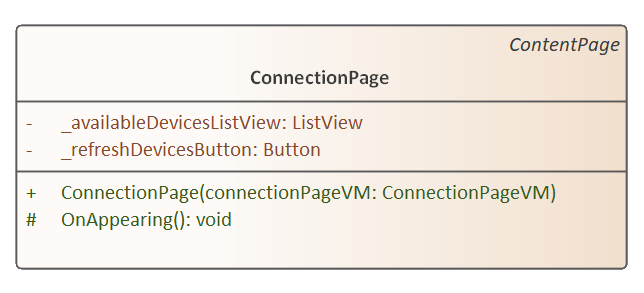
\includegraphics[page=1,width=350pt,keepaspectratio]{../uml_klassen/View/ConnectionPage.png}
\end{center}
\paragraph{Attribute}
\begin{itemize}
	\i{private ConnectionPageVM \_connectionPageVM} ViewModel der ConnectionPage
	\i{private ListView \_availableDevicesListView} Zeigt verfügbare eSense Earables an. Durch Drücken auf ein Element aus der Liste wird sich dem dem ausgewählten Earables verbunden. 
	\i{private Button \_refreshDevicesButton} Durch Drücken aktualisiert sich die Liste der verfügbaren eSense Earables
\end{itemize}

\paragraph{Methoden}
\begin{itemize}
	\i{public ConnectionPage(ConnectionPageVM connectionPageVM)} Initialisiert \_connectionPageVM und setzt den Binding Context 			auf \_connectionPageVM
	\i{protected override void OnAppearing()} Verhalten der Seite unmittelbar bevor sie angezeigt wird
\end{itemize}

\subsection{AddSongPage}
Zeigt ein Menü zum hinzufügen eines neuen Songs an.  
\begin{center}
	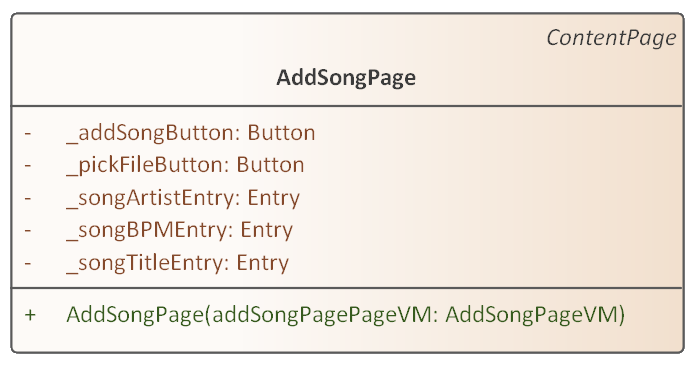
\includegraphics[page=1,width=350pt,keepaspectratio]{../uml_klassen/View/AddSongPage.png}
\end{center}
\paragraph{Attribute}
\begin{itemize}
	\i{private AddSongPageVM \_addSongPageVM} ViewModel der AddSongPage
	\i{private Entry \_songTitleEntry} Eingabefeld für den Namen des neuen Titel
	\i{private Entry \_songArtistEntry} Eingabefeld für den Künstler des neuen Titel
	\i{private Entry \_songBPMEntry} Eingabefeld für die BPM des neuen Titel
	\i{private Button \_pickFileButton} Durch Drücken öffnet sich eine Menü in dem der User einen Song aus seinem Dateiverzeichnis auswählen kann
	\i{private Button \_addSongButton} Durch Drücken wird der eingelesene Titel der Audiobibliothek hinzugefügt
\end{itemize}

\paragraph{Methoden}
\begin{itemize}
	\i{public AddSongPage(AddSongPageVM addSongPageVM)} Initialisiert \_addSongPageVM und setzt den Binding Context 			auf \_addSongPageVM
	\i{protected override void OnAppearing()} Verhalten der Seite unmittelbar bevor sie angezeigt wird
\end{itemize}

\subsection{AudioLibPage}
Zeigt die abspielbaren Titel in der AudioLibrary an.
\begin{center}
	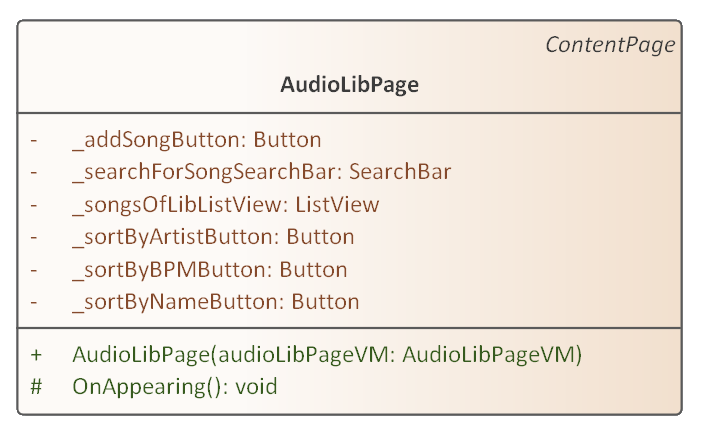
\includegraphics[page=1,width=350pt,keepaspectratio]{../uml_klassen/View/AudioLibPage.png}
\end{center}
\paragraph{Attribute}
\begin{itemize}
	\i{private AudioLibPageVM \_audioLibPageVM} ViewModel der AudioLibPage
	\i{private Button \_addSongButton} Durch Drücken wird zur AddSongPage gewechselt
	\i{private SearchBar \_searchForSongSearchBar} Bei Texteingabe der ListView aktualisiert und es werden nur noch Songs angezeigt, die das eingegebene Wort enthalten
	\i{private ListView \_songsOfLibListView} Zeigt die verfügbaren Lieder in der Audiobibliothek an
	\i{private Button \_sortByNameButton} Sortiert die Elemente des \_songsOfLibListView alphabetisch nach Name
	\i{private Button \_sortByArtistButton} Sortiert die Elemente des \_songsOfLibListView nach alphabetisch nach Künstler
	\i{private Button \_sortByBPMButton} Sortiert die Elemente des \_songsOfLibListView nach Wert der BPM (aufsteigend)
\end{itemize}

\paragraph{Methoden}
\begin{itemize}
	\i{public AudioLibPage(AudioLibPageVM audioLibPageVM)} Initialisiert \_audioLibPageVM und setzt den Binding Context 			auf \_audioLibPageVM
	\i{protected override void OnAppearing()} Verhalten der Seite unmittelbar bevor sie angezeigt wird
\end{itemize}

\subsection{AudioPlayerPage}
Zeigt einen Audioplayer an.
\begin{center}
	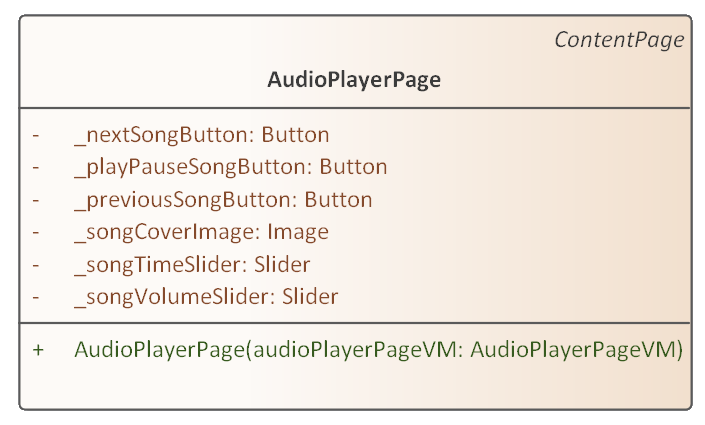
\includegraphics[page=1,width=350pt,keepaspectratio]{../uml_klassen/View/AudioPlayerPage.png}
\end{center}
\paragraph{Attribute}
\begin{itemize}
	\i{private AudioPlayerPageVM \_audioPlayerPageVM} ViewModel der AudioPlayerPage
	\i{private Image \_songCoverImage} Zeigt das Cover des abzuspielenden Lieds an
	\i{private Slider \_songTimeSlider} Zeigt die Position im abzuspielenden Lied an
	\i{private Button \_previousSongButton} Durch Drücken wird das vorherige Lied abgespielt
	\i{private Button \_playPauseSongButton} Durch Drücken wird das aktuell geladene Lied pausiert/abgespielt
	\i{private Button \_nextSongButton} Durch Drücken wird das nächste Lied abgespielt
	\i{private Slider \_songVolumeSlider} Zeigt die Lautstärke des abzuspielenden Lied an
\end{itemize}

\paragraph{Methoden}

\begin{itemize}
	\i{public AudioPlayerPage(AudioPlayerPageVM audioPlayerPageVM)} Initialisiert \_audioPlayerPageVM und setzt den Binding Context 			auf \_audioPlayerPageVM
	\i{protected override void OnAppearing()} Verhalten der Seite unmittelbar bevor sie angezeigt wird
\end{itemize}

\subsection{ModesPage}
Zeigt ein Menü zum aktivieren/deaktivieren aller Modi an.
\begin{center}
	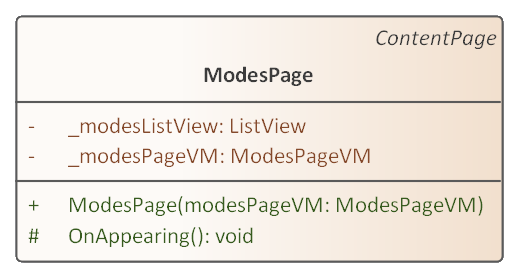
\includegraphics[page=1,width=350pt,keepaspectratio]{../uml_klassen/View/ModesPage.png}
\end{center}
\paragraph{Attribute}
\begin{itemize}
	\i{private ModesPageVM \_modesPageVM} ViewModel der ModesPage
	\i{private ListView \_modesListView} Zeigt alle verfügbaren Modi an. Die hinzufügbaren ListCells bestehen aus dem Namen des Modus und einem Switch mit dem man den Modus aktivieren kann
\end{itemize}

\paragraph{Methoden}

\begin{itemize}
	\i{public ModesPage(ModesPageVM modesPageVM)} Initialisiert \_modesPageVM und setzt den Binding Context 			auf \_modesPageVM
	\i{protected override void OnAppearing()} Verhalten der Seite unmittelbar bevor sie angezeigt wird
\end{itemize}

\subsection{SettingsPage}
Zeigt ein Menü zum Verändern der Einstellungen der App an.
\begin{center}
	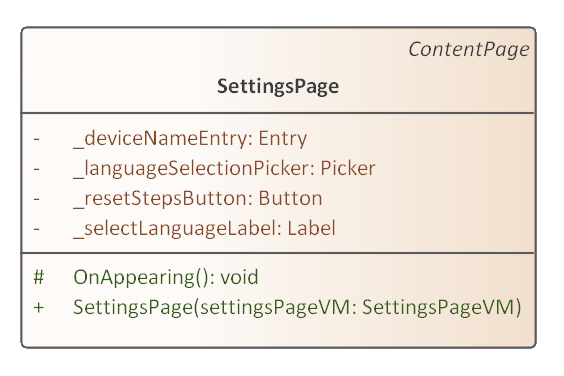
\includegraphics[page=1,width=350pt,keepaspectratio]{../uml_klassen/View/SettingsPage.png}
\end{center}
\paragraph{Attribute}

\begin{itemize}
	\i{private SettingsPageVM \_settingsPageVM} ViewModel der SettingsPage
	\i{private Entry \_deviceNameEntry} Eingabefeld für den Gerätenamen
	\i{private Label \_selectLanguageLabel} Zeigt den Text "Select Language" (in der gewählten Sprache) an
	\i{private Picker \_languageSelectionPicker} Picker für Sprachauswahl
	\i{private Button \_resetStepsButton} Durch Drücken wird die auf der MainPage anzeigte Schrittzahl auf 0 zurückgesetzt
\end{itemize}

\paragraph{Methoden}

\begin{itemize}
	\i{public SettingsPage(SettingsPageVM settingsPageVM)} Initialisiert \_settingsPageVM und setzt den Binding Context 			auf \_settingsPageVM
	\i{protected override void OnAppearing()} Verhalten der Seite unmittelbar bevor sie angezeigt wird
\end{itemize}

\end{document}
